% arara: lualatex
% arara: makeglossaries
% arara: lualatex
% arara: biber
% arara: lualatex
% arara: lualatex

% Demo report and presentation prepared by Aaron English (humdrumcomet on github)
\documentclass[hidelinks, float=false, crop=false]{article}

\usepackage{import}
\usepackage{indentfirst}
\usepackage[doublespacing]{setspace}
\usepackage{xurl}
\usepackage{hyperref}
\usepackage[tbtags]{amsmath}
\usepackage{amsfonts}
\usepackage{amssymb}
\usepackage{fancyhdr}
\usepackage[T1]{fontenc}
\usepackage{xparse}
\usepackage{xcolor}
\usepackage{colortbl}
\usepackage{siunitx}
\usepackage{chemformula}
\usepackage[style=ieee,backend=biber]{biblatex}
\usepackage{float}
\usepackage{enumitem}
\usepackage{graphicx}

\usepackage{tikz}
    \usetikzlibrary{math, arrows, circuits.ee.IEC, positioning, shapes.arrows, shapes.geometric, external}
\usepackage{pgfplots}
    \pgfplotsset{compat=newest, compat/show suggested version=false}
    \usepgfplotslibrary{groupplots}
\usepackage[siunitx,american voltages, american currents, RPvoltages]{circuitikz}

\usepackage[titles]{tocloft}
\usepackage{xpatch}
\usepackage[debug, toc, section=section, acronym, symbols]{glossaries} % Glossaries package

%Get rounded wire jumps
\tikzset{
    declare function={% in case of CVS which switches the arguments of atan2
        atan3(\a,\b)=ifthenelse(atan2(0,1)==90, atan2(\a,\b), atan2(\b,\a));},
        kinky cross radius/.initial=+.125cm,
        @kinky cross/.initial=+, kinky crosses/.is choice,
        kinky crosses/left/.style={@kinky cross=-},kinky crosses/right/.style={@kinky cross=+},
        kinky cross/.style args={(#1)--(#2)}{
        to path={
          let \p{@kc@}=($(\tikztotarget)-(\tikztostart)$),
              \n{@kc@}={atan3(\p{@kc@})+180} in
          -- ($(intersection of \tikztostart--{\tikztotarget} and #1--#2)!%
                 \pgfkeysvalueof{/tikz/kinky cross radius}!(\tikztostart)$)
          arc [ radius     =\pgfkeysvalueof{/tikz/kinky cross radius},
                start angle=\n{@kc@},
                delta angle=\pgfkeysvalueof{/tikz/@kinky cross}180 ]
          -- (\tikztotarget)}}
      }

% A new command for less cramped nested fractions
\newcommand\ddfrac[2]{\frac{\displaystyle #1}{\displaystyle #2}}
% Front matter, main matter, and back matter definitions
\def\frontmatter{%
 \pagenumbering{roman}
 \setcounter{page}{1}
 \renewcommand{\thesection}{\roman{section}}
}%
\def\mainmatter{%
 \pagenumbering{arabic}
 \setcounter{page}{1}
 \setcounter{section}{0}
 \renewcommand{\thesection}{\arabic{section}}
}%
\def\backmatter{%
 \setcounter{section}{0}
 \renewcommand{\thesection}{\alph{section}}
}%

% SI unit pkg conf
\sisetup{
    load-configurations = abbreviations,
    detect-family = true,
    per-mode = reciprocal
}%
\DeclareSIUnit{\torr}{Torr}

% Bibliography .bib file locations should maybe be local?
\addbibresource[location=local]{./accelerators.bib}

% Fancyhdr modification of page numbering
\pagestyle{fancy}
\fancyhf{}
\fancyfoot[R]{\thepage}
\renewcommand{\headrulewidth}{0pt}
\renewcommand{\footrulewidth}{1pt}
% Add Constants list using glossary
\newglossary[cgls]{constants}{cstog}{cstig}{Constants}
% Alphabetize glossary and acronyms list
\makeglossaries

%%% Constants
%%%%%%%%%%%%%%%%%%%%%%%%%%%%%%%%%%%%%%%%%%%%%%%%%%%%%%%%%%%%%%%%%%%%%%%%%%%%%%%%%%%%%%%%
\newglossaryentry{c}
{
    type=constants,
    name={\ensuremath{c}},
    description={\mbox{} speed of light (\SI{2.997924e8}{\meter\per\second})}
}
\newglossaryentry{boltz}
{
    type=constants,
    name={\ensuremath{k_{B}}},
    description={\mbox{} Boltzmann constant (\SI{8.617330e-5}{\electronvolt\per\kelvin})}
}
\newglossaryentry{eps0}
{
    type=constants,
    name={\ensuremath{\varepsilon_{0}}},
    description={\mbox{} permittivity of free space (\SI{8.854187e-12}{\farad\per\meter})}
}
\newglossaryentry{eq}
{
    type=constants,
    name={\ensuremath{e}},
    description={\mbox{} elementary charge (\SI{1.602176e-19}{\coulomb})}
}

%%% Symbols
%%%%%%%%%%%%%%%%%%%%%%%%%%%%%%%%%%%%%%%%%%%%%%%%%%%%%%%%%%%%%%%%%%%%%%%%%%%%%%%%%%%%%%%%
\newglossaryentry{mg}
{
    type=symbols,
    name={\ensuremath{G}},
    description={Mosfet Gate}
}
\newglossaryentry{md}
{
    type=symbols,
    name={\ensuremath{D}},
    description={Mosfet Drain}
}
\newglossaryentry{ms}
{
    type=symbols,
    name={\ensuremath{S}},
    description={Mosfet Source}
}
\newglossaryentry{press}
{
    type=symbols,
    name={\ensuremath{P}},
    description={Pressure (units of \si{\torr})}
}
\newglossaryentry{time}
{
    type=symbols,
    name={\ensuremath{t}},
    description={time (units of minutes)}
}
\newglossaryentry{ener}
{
    type=symbols,
    name={\ensuremath{E}},
    description={Energy}
}
\newglossaryentry{efermi}
{
    type=symbols,
    name={\ensuremath{E_{f}}},
    description={Fermi Energy of a Material}
}
\newglossaryentry{fermiDist}
{
    type=symbols,
    name={\ensuremath{f(E)}},
    description={The Fermi-Dirac distribution}
}
\newglossaryentry{econd}
{
    type=symbols,
    name={\ensuremath{E_{C}}},
    description={Conduction band energy level}
}
\newglossaryentry{evalence}
{
    type=symbols,
    name={\ensuremath{E_{V}}},
    description={Valence band energy level}
}
\newglossaryentry{egap}
{
    type=symbols,
    name={\ensuremath{E_{G}}},
    description={Bandgap}
}
\newglossaryentry{rd}
{
    type=symbols,
    name={\ensuremath{R_{D}}},
    description={Resistance}
}
\newglossaryentry{vout}
{
    type=symbols,
    name={\ensuremath{V_{out}}},
    description={Output voltage}
}
\newglossaryentry{vin}
{
    type=symbols,
    name={\ensuremath{V_{in}}},
    description={Input voltage}
}
\newglossaryentry{temp}
{
    type=symbols,
    name={\ensuremath{T}},
    description={Temperature in units of Kelvin}
}

%%%%%%%%%%%%%%%%%%%
%%%%%%%%%%%%%%%% Acronym Only
\newglossaryentry{ndfeb}
{
    type=\acronymtype,
    name={NdFeB},
    description={Neodymium Iron Boron Rare Earth Permanent Magnet},
    first={Neodymium iron boron (NdFeB)}
}
\newglossaryentry{smco}
{
    type=\acronymtype,
    name={SmCo},
    description={Samarium Cobalt Rare Earth Permanent Magnet},
    first={Samarium cobalt (SmCo)}
}
\newglossaryentry{cnc}
{
    type=\acronymtype,
    name={CNC},
    description={Computer Numerically Controlled},
    first={Computer Numerically Controlled (CNC)}
}
\newglossaryentry{ptfe}
{
    type=\acronymtype,
    name={PTFE},
    description={Polytetraflouroethylene (PTFE), commonly referred to by the brand name Teflon, is a synthetic polymer with highly desirable electrical breakdown characteristics},
    first={Polytetraflouroethylene (PTFE)}
}

%%%%%%%%%%%%%%%%%%%
%%%%%%%%%%%%%%%% Glossary Only
\newglossaryentry{cpp}
{%
    name={C++},
    description={C++ is a programming language that can be used as an object oriented programming language, an imperative programming language, and still provide low-level memory control. Note: All C++ code used in this work is compiled under the C++11 standard}
}
\newglossaryentry{python}
{%
    name={Python},
    description={Python is a flexible scripting language that can be used as an imperative language, an object oriented language. Note: All python code used in this work is written and executed using Python3.6}
}
\newglossaryentry{ibsimu}
{%
    name={IBSIMU},
    description={IBSIMU is a \gls{cpp} library for ion optics, space-charge calculation, and plasma extraction. It is able to import 2-D and 3-D geometries as exported in .STL or .DXF file formats. It also allows for mathematical definition of geometries. Note: Version 1.0.6 of the IBSIMU library was used for this work \cite{acc:14}}
}
\newglossaryentry{ansys}
{
    name={ANSYS},
    description={ANSYS Multiphysics is a software suite for multiphysics modelling and simulation}
}

%%%%%%%%%%%%%%%%%%%
%%%%%%%%%%%%%%%% Glossary and Acronym
\newglossaryentry{hvag}
{%
 name={HV},
 description={High Vacuum (HV) is a term which refers to vacuum pressures in the range of \SI{1e-3}{\torr} to \SI{1e-8}{\torr}\cite{acc:13}}
}
\newglossaryentry{hva}
{%
 type=\acronymtype,
 name={HV},
 description={High Vacuum},
 first={High Vacuum (HV)\glsadd{hvag}},
 see=[Glossary:]{hvag}
}

\begin{document}{}
    \begin{center}
        \vspace*{1cm}
        {\fontsize{30}{50}\selectfont {\bfseries Hello Again \LaTeX\\}}
        \vspace{3cm}
        {\LARGE More Capabilities of the\\
        Typesetting Tool\\}
        \vspace{7cm}
    \end{center}
    \begin{raggedleft}
        {\Large Aaron English\\
            Date: \today\\}
    \end{raggedleft}
    \thispagestyle{empty}

    \clearpage
    \tableofcontents
    \clearpage
    \section{Where Did We Leave Off?}
        Last time we talked about how \LaTeX~makes things easier for you in a number of ways, and 
        how it has many tools and packages to simplify things like page numbering, section numbering,
        references, bibliographies, figure and equation numbering, and more. 

        Now one thing that I'd like to point out is the idea that a lot of what was spoken about
        last time was often in reference to a text editor like MS-Word. So, fundamentally our 
        conversation had an implicit basis in Word's abilities and usage. 

        So this time, let's try a different approach. If our typesetting tool (this is actually what
        \LaTeX~is) has a complete programming language underneath how many things can we automate?
        Described as one of the most sophisticated typesetting programs in existence.

    \section{The Glossaries Package}
        In \LaTeX~there are a handful of packages that are \textbf{\textit{BIG}}. One such example
        is the glossaries package. It provides a great many functions, that can really change how
        you might interact with your document. 

        In short the glossaries package gives you the ability to define glossary terms, acronyms, 
        even symbols and then use them in your document and guarantee consistency and even the proper
        "first time fill version" rule for acronyms.

        Lets start with a simple example. Here I've defined a glossary term for \gls{cpp}. Not 
        too fancy, but this now is a link to the glossary, where the confused reader can go for more
        information. As a bonus, once you've defined your glossary term, if you decide it should look 
        different, you only need to change it in one place, and your changes propagate through the
        whole document.
        
        Now let's get a little fancier. How about an acronym, something like \gls{cnc}. The first time
        I mention it, it shows up as the full name. The second time I mention \gls{cnc}, only the 
        acronym shows up! Of course it doesn't matter if the order changes, \LaTeX~will always get it 
        right (almost, watch out for using it in titles). This can also be combined with a glossary,
        for the instances where you're trying to expand on the acronym. So say for example I'm talking
        about \gls{hva}. The acronym for \gls{hva} is just simply expanded to \glsdesc{hva},
        so then now I can add a glossary term and have the two linked, giving me greater expandability.

        Now I know not everyone is in need of glossaries for the projects or reports but I assure you
        this package is worth it for more reasons than just the acronyms and the glossaries, because
        you could even use it to define symbols and constants, and then use those in equations.

        Lets take an example and write out the equation for the Fermi-Dirac distribution, Equation \ref{eqt:fermiDirac}.

        \begin{equation}
            \gls{fermiDist} = \left(e^{\left(\ddfrac{\gls{ener}-\gls{efermi}}{\gls{boltz}\gls{temp}}\right)}+1\right)^{-1}
            \label{eqt:fermiDirac}
        \end{equation}

        As you can see, we know can enforce consistent notation, and if later on we decide we'd like 
        to change the notation, we only have to go to one place.
        

    \section{Vector and Raster Graphics}
        Did you ever notice that when you zoom in on the letters in a PDF file, they never pixelate?
        But this is not true of your graphics when you add them to your documents? Well this has
        to do with the difference between vector and raster graphics. 

        Roughly speaking vector graphics are equation based. They are graphics defined by points 
        connected by lines and curves. Because they are equation based, they can be zoomed into
        arbitrarily. Raster graphics on the other hand are defined instead in terms of pixels and 
        so do not provide the same benefits and scalability as vector graphics.

        So what if you wanted your graphics in your reports to be vector based? What if you wanted
        your figures to match the font and style of the rest of the report? 

        Well this can all be accomplished with another one of the large behaviour changing \LaTeX~
        packages. This one is called TikZ, and I'll show you a few examples of things you can do
        with it.

        \subsection{TikZ}
            TikZ is extremely powerful. It can create anything you want to display, but it does have
            a bit of a learning curve. First let's talk about what you could accomplish with it.

            One fantastic aspect of TikZ is that it integrates seamlessly with the rest of your
            document. The same fonts, the same symbols, and even, clean integration with glossaries
            giving you all the benefits explored before. 

            \begin{figure}[htbp]
                \begin{centering}
                    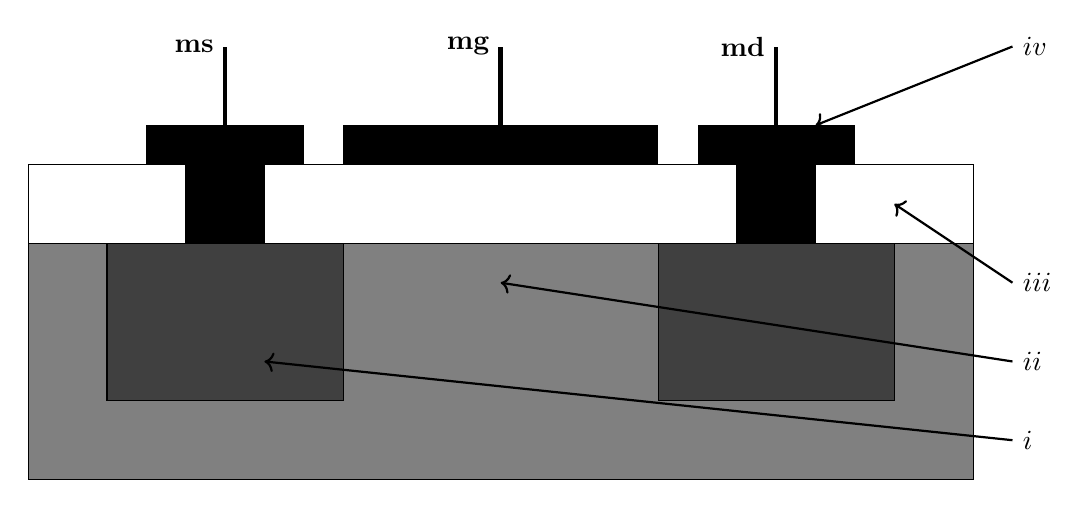
\begin{tikzpicture}
                        \draw[fill=gray] (0,0) rectangle (12,3);
                        \draw[fill=darkgray] (1,1) rectangle (4,3);
                        \draw[fill=darkgray] (8,1) rectangle (11,3);
                        \draw (3,3) rectangle (9, 4);
                        \draw (0,3) rectangle (2,4);
                        \draw (10,3) rectangle (12,4);
                        \fill[black] (4,4) rectangle (8,4.5);
                        \fill[black] (2,3) rectangle (3,4.5);
                        \fill[black] (1.5,4) rectangle (3.5,4.5);
                        \fill[black] (9,3) rectangle (10,4.5);
                        \fill[black] (8.5,4) rectangle (10.5,4.5);
                        \draw[ultra thick] (2.5,4.5)--(2.5,5.5)node[left]{\bf \gls{ms}};
                        \draw[ultra thick] (6,4.5)--(6,5.5)node[left]{\bf \gls{mg}};
                        \draw[ultra thick] (9.5,4.5)--(9.5,5.5)node[left]{\bf \gls{md}};
                        \draw[thick, <-] (10,4.5)--(12.5,5.5)node[right]{\bf $iv$};
                        \draw[thick, <-] (11,3.5)--(12.5,2.5)node[right]{\bf $iii$};
                        \draw[thick, <-] (6,2.5)--(12.5,1.5)node[right]{\bf $ii$};
                        \draw[thick, <-] (3,1.5)--(12.5,0.5)node[right]{\bf $i$};
                    \end{tikzpicture}
                    \caption{A simple TikZ diagram showing a MOSFET}
                    \label{fig:tikzFET}
                \end{centering}
            \end{figure}

            These are just a few examples of the sorts of things you can create with TikZ that show
            the integration with the rest of the typical \LaTeX~utilities.

            \begin{figure}[htbp]
                \begin{centering}
                    \begin{tikzpicture}
                        \draw[->] (0,0)--(13,0) node[below right]{$x$};
                        \draw[->] (0,0)--(0,7.5) node[left]{\gls{ener}};
                        \draw (0,6.5)node[left]{\gls{econd}}--(4,6.5);
                        \draw (8,4)--(12,4) node[right]{\gls{econd}};
                        \draw (4,6.5) to [out=0, in=180] (8,4);
                        \draw (0,3)node[left]{\gls{evalence}}--(4,3);
                        \draw (8,0.5)--(12,0.5) node[right]{\gls{evalence}};
                        \draw (4,3) to [out=0, in=180] (8,0.5);
                        \draw[dashed] (0,3.5)node[left]{$\gls{efermi}_{p}$}--(12,3.5)node[right]{$\gls{efermi}_{n}$};
                        \draw[dashed] (6,0)--(6,6.5)node[above]{$PN-Junction$};
                        \draw[<->] (11,0.5)--(11,4);
                        \node[right]  at (11,2.5){\gls{egap}};
                        \node at (2,1.5){$P-Type$};
                        \node at (10,5.5){$N-Type$};
                    \end{tikzpicture}
                    \caption{A simple Example TikZ showing the band diagram of a PN-junction}
                    \label{fig:diodeBandBend}
                \end{centering}
            \end{figure}

            \begin{figure}[htbp]
                \begin{centering}
                        \begin{tikzpicture}
                            \draw[->] (0,0)--(0,6.5)node[left]{\gls{ener}};
                            \draw[->] (0,0)--(5.5,0)node[right]{\gls{fermiDist}};
                            \draw[dashed] (2.5,0)node[below]{$\sfrac{1}{2}$}--(2.5,3);
                            \draw[dashed] (0,3)node[left]{\gls{efermi}}--(2.5,3);
                            \draw (0.05,6)--(0.05,4.5);
                            \draw (0.05,4.5) to [out=270, in=90] (5,1.5);
                            \draw (5,1.5)--(5,0)node[below]{$1$};
                            \draw (0.05,6)--(0.05,5.5);
                            \draw (0.05,5.5) to [out=270, in=90] (5, 0.5);
                            \draw (5,0.5)--(5,0);
                            \draw[->] (0.3,3.3)--(2,4.5)node[right]{$\gls{temp}_{increasing}$};
                        \end{tikzpicture}
                    \caption{A TikZ Diagram showing a sketch of the Fermi-Dirac distribution}
                    \label{fig:tikzFDDist}
                \end{centering}
            \end{figure}
            
        \subsection{Pgfplots}
            Great plots, consistent visuals, not too hard to implement.
            \begin{figure}[htbp]
                \begin{centering}
                    \begin{tikzpicture}
                        \begin{axis}[ymode=log,
                            grid=both,
                            ymin=1e-6,
                            ymax=1e3,
                            max space between ticks=30,
                            xmin=0,
                            xmax=350,
                            xlabel=\gls{time},
                            ylabel=\gls{press},
                            title=Chamber Pressure over Time]
                            \addplot[color=red, mark size=0.4, style=thick]table[x=time, y=p1, col sep=comma]{./vacuumTech.csv};
                            \addplot[color=black, mark=*, mark size=0.4, style=thick]table[x=time, y=p2, col sep=comma]{./vacuumTech.csv};
                        \end{axis}
                    \end{tikzpicture}
                    \caption{A TikZ plot from some data in a CSV file}
                    \label{fig:tikzPlot}
                \end{centering}
            \end{figure}
            
        \subsection{CircuitTikZ}
            There are even TikZ modules for the creation of circuit diagrams. Again, all the same
            abilities you know and love are available to you.

            \begin{figure}[htbp]
                \begin{centering}
                    \begin{circuitikz}[voltage shift=0.5]
                        \draw (0, 0) node[nigbt,](Q1){};
                        \draw (Q1.E) -- ++(0, -2) node[nigbt,anchor=C](Q2){};
                        \draw (Q2.E) -- ++(0,-1) -- ++(-3,0) node[shape=ground]{} to[V,l=\gls{vin}] ++(0,7) --
                                ++(3, 0) coordinate(int1) to[short] (Q1.C);

                        \draw (Q1.C) ++(2, 0) node[nigbt,anchor=C](Q3){};
                        \draw (Q3.E) -- ++(0, -2) node[nigbt,anchor=C](Q4){};
                        \draw (Q4.E) -- ++(0,-1) -- ++(-2,0) node[circ]{};
                        \draw (int1) node[circ]{} -- ++(2,0) -- (Q3.C);

                        \draw (Q1.E) node[circ]{} to[kinky cross=(Q3.E)--(Q4.C)] ++(3,0) coordinate(Trans1);

                        \draw (Trans1) node[transformer core, anchor=A1, circuitikz/inductors/coils=6](T){}
                                (T.base) node[above]{$N_{1}:N_{2}$};
                        \draw (T.A2) -- ++(-1,0) node[circ]{};
                        
                        \draw (T.B1) to[D,] ++(2,0) coordinate(vout) node[circ]{} -- ++(1.5,0)
                        node[circ]{} coordinate(cout) -- ++(1,0)coordinate (rout) to[R=,v^=\gls{vout}] 
                                (rout |- T.B2) -- ++(-1,0) coordinate(end) node[circ]{} to [C,] (cout);
                        \draw (T-L2.midtap) to[short] ++(3,0) coordinate(mid) -- (mid |- T.B2) -- (end);
                        \draw (T.B2) to[D,] ++(2,0) to[kinky cross=(T-L2.midtap)--(mid)] (vout);
                    \end{circuitikz}
                    \caption{An Example of a circuit (an isolated boost converter) done in circuit TikZ}
                    \label{fig:circuitTikZ}
                \end{centering}
            \end{figure}
            
    
    \section{What Next?}
        So far we've talked about all these different aspects of how you can accomplish so many
        things in \LaTeX, but what about presentations? What do we do when we need a slideshow?
        Well, of course, there is an answer and that answer is Beamer.

    \clearpage
    \printglossaries
\end{document}
